% Compile with: xelatex dunnhumby_dataset_selection.tex (run twice)
\documentclass[aspectratio=169,11pt]{beamer}

\usepackage{fontspec}
\IfFontExistsTF{Noto Sans}{
  \setsansfont{Noto Sans}
}{
  \IfFontExistsTF{Arial}{\setsansfont{Arial}}{\setsansfont{TeX Gyre Heros}}
}
\usepackage{booktabs}
\usepackage{tabularx}
\usepackage{array}
\usepackage{ragged2e}
\usepackage{tikz}
\usetikzlibrary{arrows.meta,calc,positioning,shapes.geometric}
\usepackage{appendixnumberbeamer}

\definecolor{Navy}{HTML}{17365D}
\definecolor{Blue}{HTML}{2F75B5}
\definecolor{Teal}{HTML}{00A6A6}
\definecolor{Orange}{HTML}{ED7D31}
\definecolor{Green}{HTML}{70AD47}
\definecolor{LightBlue}{HTML}{DDEBF7}
\definecolor{LightTeal}{HTML}{DDEFEF}
\definecolor{LightGray}{HTML}{F2F2F2}
\definecolor{DarkGray}{HTML}{404040}

\usetheme{default}
\setbeamertemplate{navigation symbols}{}
\setbeamercolor{normal text}{fg=DarkGray,bg=white}
\setbeamercolor{structure}{fg=Navy}
\setbeamercolor{frametitle}{fg=white,bg=Navy}
\setbeamerfont{frametitle}{series=\bfseries,size=\large}
\setbeamercolor{title}{fg=white}
\setbeamercolor{subtitle}{fg=LightBlue}
\setbeamercolor{block title}{fg=white,bg=Blue}
\setbeamercolor{block body}{fg=DarkGray,bg=LightBlue}
\setbeamercolor{alerted text}{fg=Orange}
\setbeamertemplate{itemize item}{\color{Teal}$\blacktriangleright$}
\setbeamertemplate{itemize subitem}{\color{Blue}$\bullet$}
\setbeamertemplate{enumerate item}{\color{Teal}\insertenumlabel.}
\setbeamertemplate{footline}{%
  \leavevmode%
  \hbox{%
    \begin{beamercolorbox}[wd=.78\paperwidth,ht=2.6ex,dp=1.1ex,leftskip=1em]{author in head/foot}%
      \color{DarkGray}\small Customer Purchase Propensity --- Dataset Selection
    \end{beamercolorbox}%
    \begin{beamercolorbox}[wd=.22\paperwidth,ht=2.6ex,dp=1.1ex,rightskip=1em plus1fil]{date in head/foot}%
      \color{Navy}\small\hfill \insertframenumber/\inserttotalframenumber
    \end{beamercolorbox}%
  }%
}
\setbeamertemplate{headline}{}

\newcommand{\source}[1]{\vspace{0.2em}{\tiny\color{gray}Nguồn: #1}}
\newcommand{\good}{\textcolor{Green}{\bfseries\checkmark}}
\newcommand{\weak}{\textcolor{Orange}{\bfseries$\triangle$}}
\newcommand{\bad}{\textcolor{red!70!black}{\bfseries$\times$}}
\newcommand{\score}[1]{\textbf{#1}/5}

\title{Vì sao chọn Dunnhumby\newline cho bài toán Customer Purchase Propensity?}
\subtitle{Từ yêu cầu kinh doanh đến bằng chứng dữ liệu và khả năng triển khai}
\author{Tên người trình bày: \textbf{[Điền tên]}}
\institute{Đơn vị: \textbf{[Điền phòng ban / công ty]}}
\date{Ngày báo cáo: \textbf{[Điền ngày]}}

\begin{document}

% -----------------------------------------------------------------------------
\begin{frame}[plain]
  
\begin{tikzpicture}[remember picture,overlay]
    \fill[Navy] (current page.south west) rectangle (current page.north east);
    \fill[Teal] (current page.south west) rectangle
      ([xshift=0.18\paperwidth]current page.north west);
    \fill[Orange] ([yshift=0.08\paperheight]current page.south west) rectangle
      ([yshift=0.095\paperheight]current page.south east);
  \end{tikzpicture}
  \vspace{1.2cm}
  \hspace{1.6cm}
  \begin{minipage}{0.78\textwidth}
    {\usebeamerfont{title}\color{white}\LARGE\bfseries\inserttitle\par}
    \vspace{0.55cm}
    {\color{LightBlue}\large\insertsubtitle\par}
    \vspace{1.1cm}
    {\color{white}\insertauthor\par}
    {\color{white}\insertinstitute\par}
    {\color{white}\insertdate\par}
  \end{minipage}
  \note{Mở đầu bằng câu hỏi lựa chọn dữ liệu, không mở đầu bằng mô hình. Nhấn mạnh rằng
  mục tiêu hôm nay là bảo vệ tính phù hợp của Dunnhumby trước khi trình bày kết quả ML.}
\end{frame}

% -----------------------------------------------------------------------------
\begin{frame}{Thông điệp chính}
  \begin{columns}[T,onlytextwidth]
    \column{0.31\textwidth}
      \begin{block}{Đúng grain}
        Household $\rightarrow$ basket $\rightarrow$ product, có hành vi lặp theo thời gian.
      \end{block}
    \column{0.31\textwidth}
      \begin{block}{Đủ context}
        Transaction, product, promotion, campaign và một phần demographic.
      \end{block}
    \column{0.31\textwidth}
      \begin{block}{Dựng được target}
        Feature trước cutoff; purchase label sau cutoff; đánh giá theo thời gian.
      \end{block}
  \end{columns}
  \vspace{0.65cm}
  \begin{center}
    \begin{tikzpicture}
      \node[draw=Navy,fill=LightBlue,rounded corners=6pt,inner sep=10pt,
        text width=.86\textwidth,align=center] {
        \Large\bfseries Dunnhumby không chỉ ``lớn''; dataset này phù hợp với
        \alert{đúng quyết định kinh doanh} của customer purchase propensity.
      };
    \end{tikzpicture}
  \end{center}
  \note{Đây là kết luận cần khán giả nhớ. Ba tiêu chí là grain, context và temporal
  constructibility. Quy mô chỉ là điều kiện hỗ trợ, không phải lý do chính.}
\end{frame}

% -----------------------------------------------------------------------------
\begin{frame}{Bài toán cần dữ liệu như thế nào?}
  \begin{columns}[T,onlytextwidth]
    \column{0.52\textwidth}
      \textbf{Câu hỏi dự báo}
      \[
        P(\text{household mua trong 7 ngày tới}
        \mid \text{hành vi đến hôm nay})
      \]
      \vspace{0.2cm}
      \begin{alertblock}{Đơn vị quyết định}
        Một household tại một thời điểm chấm điểm --- không phải một sản phẩm
        hay một phiên truy cập riêng lẻ.
      \end{alertblock}
    \column{0.45\textwidth}
      \textbf{Yêu cầu tối thiểu của dataset}
      \begin{enumerate}
        \item Customer/household ID ổn định.
        \item Nhiều lần mua theo thời gian.
        \item Basket và thời điểm giao dịch.
        \item Lịch sử đủ dài để tạo feature/label.
        \item Biến giải thích có ý nghĩa kinh doanh.
        \item Cho phép temporal validation, không leakage.
      \end{enumerate}
  \end{columns}
  \note{Dẫn dắt từ bài toán sang tiêu chí dữ liệu. Nếu không có ID lặp hoặc thời gian,
  ta không thể dự báo propensity đúng nghĩa mà chỉ làm classification tĩnh.}
\end{frame}

% -----------------------------------------------------------------------------
\begin{frame}{Khung lựa chọn dataset --- tiêu chí được xác định trước}
  \small
  \begin{tabularx}{\textwidth}{>{\bfseries}p{3.2cm}Xc}
    \toprule
    Tiêu chí & Câu hỏi đánh giá & Trọng số \\
    \midrule
    Phù hợp business target & Có dựng được purchase propensity ở household-level? & 25\% \\
    Temporal validity & Có đủ lịch sử và timestamp để chia train/test theo thời gian? & 20\% \\
    Behavioral richness & Có recency, frequency, basket, spend, category, promotion? & 20\% \\
    Marketing context & Có campaign/coupon/direct-marketing information? & 15\% \\
    Realism và interpretability & Có giống dữ liệu retail để nói chuyện với quản lý? & 10\% \\
    Feasibility & Có thể xử lý, kiểm tra và tái lập trong phạm vi project? & 10\% \\
    \bottomrule
  \end{tabularx}
  \vspace{0.35cm}
  \begin{center}
    \color{Navy}\bfseries Không chọn dataset sau khi nhìn model score;
    chọn theo sự phù hợp với quyết định.
  \end{center}
  \note{Slide này chống cherry-picking. Nói rõ trọng số là framework của project,
  không phải benchmark học thuật tuyệt đối. Có thể điều chỉnh trọng số nếu business
  owner đổi use case.}
\end{frame}

% -----------------------------------------------------------------------------
\begin{frame}{So sánh các lựa chọn phổ biến}
  \scriptsize
  \renewcommand{\arraystretch}{1.2}
  \begin{tabularx}{\textwidth}{>{\bfseries}p{3.25cm}cccX}
    \toprule
    Tiêu chí & Dunnhumby & Instacart & UCI Online Retail & Nhận xét \\
    \midrule
    Household purchase propensity & \score{5} & \score{3} & \score{3} &
      Dunnhumby đúng household, basket và any-purchase timing. \\
    Temporal history & \score{5} & \score{4} & \score{4} &
      Cả ba có sequence; Dunnhumby có khoảng hai năm hành vi. \\
    Behavioral richness & \score{5} & \score{4} & \score{2} &
      Dunnhumby có spend, discount, store, product hierarchy. \\
    Marketing context & \score{5} & \score{1} & \score{1} &
      Dunnhumby có campaign, coupon, redemption, display/mailer. \\
    Retail realism & \score{4} & \score{4} & \score{3} &
      UCI tập trung non-store gifts và nhiều khách wholesale. \\
    Project feasibility & \score{4} & \score{4} & \score{5} &
      UCI nhẹ hơn nhưng thiếu context; Dunnhumby vẫn xử lý được. \\
    \midrule
    \textbf{Điểm có trọng số} & \textbf{4.80} & \textbf{3.30} & \textbf{2.95} &
      Thang 1--5; scoring là đánh giá theo use case của project. \\
    \bottomrule
  \end{tabularx}
  \vspace{0.2cm}
  \source{Dunnhumby Source Files; Kaggle Market Basket Analysis; UCI Online Retail.}
  \note{Instacart rất tốt cho next-product/reorder recommendation, nhưng câu hỏi gốc
  của competition là sản phẩm nào xuất hiện ở next order. UCI dễ xử lý nhưng chỉ có
  sáu feature và ít marketing context.}
\end{frame}

% -----------------------------------------------------------------------------
\begin{frame}{Dataset được thiết kế cho customer-level retail research}
  \begin{columns}[T,onlytextwidth]
    \column{0.55\textwidth}
      \begin{block}{Mô tả chính thức của Dunnhumby}
        \begin{itemize}
          \item Household-level transactions trong khoảng hai năm.
          \item 2.500 hộ frequent shoppers tại một retailer.
          \item Toàn bộ purchase trong store, không giới hạn vài category.
          \item Customer attributes và direct-marketing contact history cho một số hộ.
          \item Dùng cho advanced classroom và academic research về direct marketing.
        \end{itemize}
      \end{block}
    \column{0.42\textwidth}
      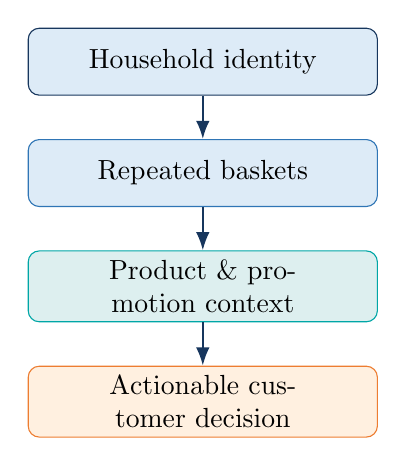
\begin{tikzpicture}[node distance=0.55cm]
        \node[draw=Navy,fill=LightBlue,rounded corners,align=center,
          text width=4.2cm,minimum height=.85cm] (h) {Household identity};
        \node[draw=Blue,fill=LightBlue,rounded corners,align=center,
          text width=4.2cm,minimum height=.85cm,below=of h] (b) {Repeated baskets};
        \node[draw=Teal,fill=LightTeal,rounded corners,align=center,
          text width=4.2cm,minimum height=.85cm,below=of b] (p) {Product \& promotion context};
        \node[draw=Orange,fill=orange!12,rounded corners,align=center,
          text width=4.2cm,minimum height=.85cm,below=of p] (d) {Actionable customer decision};
        \draw[-{Latex},thick,Navy] (h)--(b);
        \draw[-{Latex},thick,Navy] (b)--(p);
        \draw[-{Latex},thick,Navy] (p)--(d);
      \end{tikzpicture}
  \end{columns}
  \source{\href{https://www.dunnhumby.com/source-files/}{dunnhumby.com/source-files --- The Complete Journey}.}
  \note{Đây là lý do nguồn chính thức quan trọng: mục đích công bố dataset đã gần với
  bài toán nghiên cứu của project, thay vì phải ép một dataset khác vào use case.}
\end{frame}

% -----------------------------------------------------------------------------
\begin{frame}{Kiến trúc dữ liệu: một customer view đa chiều}
  \centering
  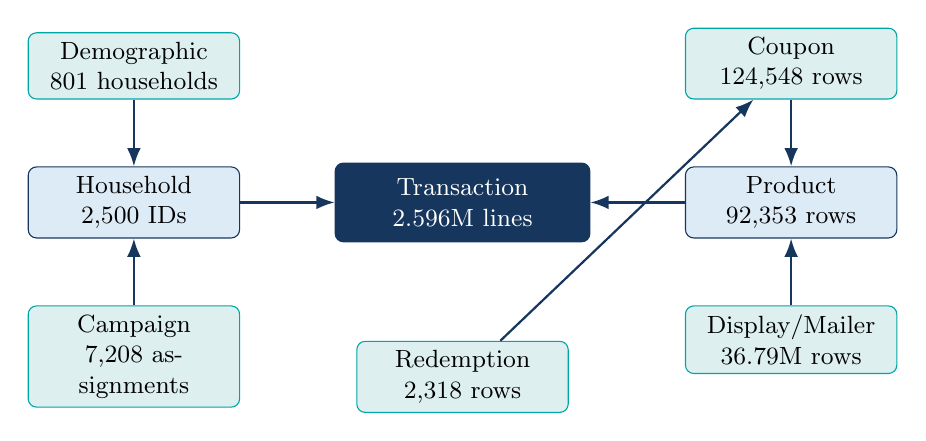
\begin{tikzpicture}[
      box/.style={draw=Navy,rounded corners=3pt,align=center,minimum height=.8cm,
        text width=2.45cm,fill=LightBlue,font=\small},
      support/.style={box,fill=LightTeal,draw=Teal},
      arrow/.style={-{Latex},thick,Navy}
    ]
    \node[box,fill=Navy,text=white,text width=3.0cm,minimum height=1.0cm] (tx)
      {Transaction\\2.596M lines};
    \node[box,left=1.2cm of tx] (hh) {Household\\2,500 IDs};
    \node[box,right=1.2cm of tx] (prod) {Product\\92,353 rows};
    \node[support,above left=.8cm and 1.2cm of tx] (demo) {Demographic\\801 households};
    \node[support,above right=.8cm and 1.2cm of tx] (coupon) {Coupon\\124,548 rows};
    \node[support,below left=.8cm and 1.2cm of tx] (campaign) {Campaign\\7,208 assignments};
    \node[support,below right=.8cm and 1.2cm of tx] (causal) {Display/Mailer\\36.79M rows};
    \node[support,below=1.25cm of tx] (redeem) {Redemption\\2,318 rows};
    \draw[arrow] (hh)--(tx);
    \draw[arrow] (prod)--(tx);
    \draw[arrow] (demo)--(hh);
    \draw[arrow] (coupon)--(prod);
    \draw[arrow] (campaign)--(hh);
    \draw[arrow] (causal)--(prod);
    \draw[arrow] (redeem)--(coupon);
  \end{tikzpicture}
  \vspace{0.3cm}
  \textbf{Ưu thế:} cùng một household có thể được nhìn qua hành vi, basket,
  assortment, promotion và marketing exposure.
  \note{Không nhất thiết dùng mọi bảng trong model đầu tiên. Giá trị nằm ở khả năng
  mở rộng use case và kiểm chứng các giả thuyết kinh doanh.}
\end{frame}

% -----------------------------------------------------------------------------
\begin{frame}{Quy mô đủ để học hành vi, vẫn đủ để audit}
  \begin{columns}[T,onlytextwidth]
    \column{0.48\textwidth}
      \begin{tabular}{lr}
        \toprule
        Thành phần & Kết quả audit \\
        \midrule
        Tổng source rows & $>$39.5 triệu \\
        Transaction lines & 2,595,732 \\
        Households & 2,500 \\
        Baskets & 276,484 \\
        Products đã mua & 92,339 \\
        Stores & 582 \\
        Khoảng thời gian & Day 1--711 \\
        Product join coverage & 100\% \\
        \bottomrule
      \end{tabular}
    \column{0.49\textwidth}
      \begin{block}{Điểm cân bằng phù hợp}
        \begin{itemize}
          \item Đủ observations để tạo nhiều snapshot cho mỗi hộ.
          \item Đủ product/category diversity để học shopping pattern.
          \item Không chỉ là một bảng đã aggregate sẵn.
          \item Vẫn có thể kiểm tra join, grain, cutoff và data-quality trên máy cá nhân.
        \end{itemize}
      \end{block}
  \end{columns}
  \source{Audit trực tiếp từ 8 CSV trong project; số liệu không lấy từ mô tả quảng bá.}
  \note{Phân biệt source description và empirical audit. Đây là con số đã đo trên file
  thực tế, giúp tăng độ tin cậy khi báo cáo.}
\end{frame}

% -----------------------------------------------------------------------------
\begin{frame}{Target có thể dựng đúng theo thời gian}
  \begin{center}
    \Large
    $P\big(Y_{h,s}=1\mid X_{h,\leq s}\big)$,
    \quad
    $Y_{h,s}=\mathbb{1}\{\text{có basket trong }(s,s+7]\}$
  \end{center}
  \vspace{0.25cm}
  \begin{tikzpicture}[x=0.82cm,y=1cm]
    \draw[very thick,Navy,-{Latex}] (0,0)--(13.2,0);
    \draw[very thick,Blue] (0,0)--(8,0);
    \draw[very thick,Orange] (8.2,0)--(12.0,0);
    \draw (8,0.18)--(8,-0.18);
    \node[above,align=center] at (4,0.1) {Feature history\\7/30/90/180 ngày};
    \node[above,align=center] at (10.1,0.1) {Label window\\7 ngày tương lai};
    \node[below] at (0,-0.05) {$s-180$};
    \node[below] at (8,-0.05) {$s$ cutoff};
    \node[below] at (12,-0.05) {$s+7$};
  \end{tikzpicture}
  \vspace{0.25cm}
  \begin{columns}[T,onlytextwidth]
    \column{0.48\textwidth}
      \begin{itemize}
        \item 75 weekly snapshots.
        \item 187,305 household-snapshot rows.
      \end{itemize}
    \column{0.48\textwidth}
      \begin{itemize}
        \item Household eligible sau first purchase.
        \item Temporal split và label embargo.
      \end{itemize}
  \end{columns}
  \note{Đây là điểm mạnh quyết định so với dataset tĩnh. Có thể tạo nhiều observation
  point-in-time mà vẫn kiểm soát leakage.}
\end{frame}

% -----------------------------------------------------------------------------
\begin{frame}{Vì sao chọn horizon 7 ngày?}
  \begin{columns}[T,onlytextwidth]
    \column{0.46\textwidth}
      \begin{tabular}{lccc}
        \toprule
        Horizon & Target rate & Min & Max \\
        \midrule
        \textbf{7 ngày} & \textbf{53.05\%} & 49.78\% & 57.14\% \\
        14 ngày & 68.26\% & 65.80\% & 71.26\% \\
        30 ngày & 80.96\% & 78.69\% & 82.99\% \\
        \bottomrule
      \end{tabular}
      \vspace{0.35cm}
      {\small Target rate trung bình và range qua weekly snapshots.}
    \column{0.50\textwidth}
      \begin{alertblock}{Lập luận lựa chọn}
        \begin{itemize}
          \item Khớp cadence ra quyết định hàng tuần.
          \item Đủ ngắn để hành động kịp thời.
          \item Positive/negative tương đối cân bằng.
          \item Horizon dài khiến phần lớn frequent shoppers trở thành positive,
            giảm giá trị phân loại audience.
        \end{itemize}
      \end{alertblock}
  \end{columns}
  \note{Đây là phân tích sensitivity, không chọn 7 ngày tùy ý. Đồng thời thừa nhận
  household là frequent shoppers nên target rate vốn cao.}
\end{frame}

% -----------------------------------------------------------------------------
\begin{frame}{Dữ liệu hỗ trợ feature có ý nghĩa kinh doanh}
  \small
  \begin{tabularx}{\textwidth}{>{\bfseries}p{3.1cm}p{4.3cm}X}
    \toprule
    Nhóm feature & Nguồn dữ liệu & Câu hỏi kinh doanh \\
    \midrule
    Recency / cadence & Household, day, basket & Hộ mua gần đây và đều đặn đến mức nào? \\
    Frequency / basket & Basket, line item & Tần suất và độ lớn chuyến mua ra sao? \\
    Monetary & Sales value & Mức chi tiêu và xu hướng thay đổi thế nào? \\
    Category / brand & Department, commodity, brand & Hộ mua grocery/fresh/private label ở mức nào? \\
    Promotion dependency & Retail/coupon discounts & Hành vi có phụ thuộc khuyến mãi không? \\
    Context / diversity & Store, time, product & Shopping pattern có đa dạng và ổn định không? \\
    Marketing history & Campaign, coupon, mailer/display & Có nền tảng để mở rộng sang campaign/uplift không? \\
    \bottomrule
  \end{tabularx}
  \vspace{0.3cm}
  \begin{center}
    \textcolor{Navy}{\bfseries Dataset cho phép đi từ RFM baseline đến feature store
    giàu ngữ nghĩa mà không đổi prediction grain.}
  \end{center}
  \note{Không nói càng nhiều feature càng tốt. Điểm quan trọng là mỗi nhóm feature gắn
  với một giả thuyết có thể giải thích cho business.}
\end{frame}

% -----------------------------------------------------------------------------
\begin{frame}{Phù hợp với câu chuyện giá trị kinh doanh}
  \begin{columns}[T,onlytextwidth]
    \column{0.50\textwidth}
      \begin{block}{Quyết định có thể hỗ trợ}
        \begin{itemize}
          \item Weekly audience prioritization khi capacity hữu hạn.
          \item Contact suppression cho nhóm xác suất thấp.
          \item Expected-purchaser planning.
          \item Chọn sample/power cho A/B test.
          \item Nền móng cho churn, next-category và uplift.
        \end{itemize}
      \end{block}
    \column{0.47\textwidth}
      \begin{alertblock}{Không được suy diễn}
        \begin{itemize}
          \item Propensity $\neq$ incremental response.
          \item Score cao không có nghĩa nên phát coupon.
          \item Offline lift không phải campaign ROI.
          \item Muốn chứng minh causal value cần randomized holdout.
        \end{itemize}
      \end{alertblock}
  \end{columns}
  \vspace{0.3cm}
  \source{Dunnhumby mô tả predictive triggers và continuous A/B testing trong customer journey communications.}
  \note{Slide này tạo sự tin cậy với quản lý: trình bày rõ giá trị nhưng không overclaim.}
\end{frame}

% -----------------------------------------------------------------------------
\begin{frame}{Không né tránh hạn chế của Dunnhumby}
  \small
  \begin{tabularx}{\textwidth}{>{\bfseries}p{3.4cm}X>{\RaggedRight\arraybackslash}p{4.6cm}}
    \toprule
    Hạn chế & Rủi ro & Cách xử lý trong project \\
    \midrule
    2,500 frequent shoppers & External validity hạn chế; target rate cao &
      Chỉ claim trong population quan sát; không suy rộng toàn retailer. \\
    Demographic coverage 32.04\% & Missing-not-at-random, segment bias &
      Giữ `Unknown`; không loại household; báo cáo segment metrics. \\
    `DAY` không có calendar date & Không chứng minh seasonality thực tế &
      Temporal order vẫn dùng được; tránh claim calendar effects. \\
    `QUANTITY` khác scale ở fuel/misc & Sai feature semantics &
      Loại raw quantity; dùng basket, line và diversity. \\
    Observational campaign data & Không xác định causal uplift &
      Propensity trước; randomized pilot/uplift là phase sau. \\
    \bottomrule
  \end{tabularx}
  \vspace{0.2cm}
  \begin{center}
    \textbf{Một dataset tốt không phải dataset hoàn hảo; đó là dataset có hạn chế
    nhìn thấy được và kiểm soát được.}
  \end{center}
  \note{Đây thường là slide được mentor đánh giá cao. Nêu hạn chế trước khi bị hỏi và
  cho thấy mỗi hạn chế đã dẫn đến một control cụ thể.}
\end{frame}

% -----------------------------------------------------------------------------
\begin{frame}{Bằng chứng hậu nghiệm: dataset thực sự học được propensity}
  \begin{columns}[T,onlytextwidth]
    \column{0.47\textwidth}
      \begin{tabular}{lr}
        \toprule
        Temporal holdout metric & Kết quả \\
        \midrule
        PR-AUC & 0.8506 \\
        ROC-AUC & 0.8303 \\
        Brier score & 0.1679 \\
        Lift @ top 10\% & 1.819x \\
        Purchase rate top 10\% & 96.80\% \\
        \bottomrule
      \end{tabular}
      \vspace{0.3cm}
      {\small 3 rolling-origin folds + final temporal holdout.}
    \column{0.49\textwidth}
      \begin{block}{Ý nghĩa đúng}
        \begin{itemize}
          \item Cadence và store/assortment diversity là signal chính.
          \item Feature từ dataset tạo được ranking ổn định theo thời gian.
          \item Kết quả xác nhận feasibility; không phải tiêu chí chọn dataset ban đầu.
        \end{itemize}
      \end{block}
  \end{columns}
  \vspace{0.25cm}
  \begin{center}
    \textcolor{Orange}{\bfseries Dataset selection được bảo vệ bằng fit-for-purpose;
    model result chỉ là validation sau cùng.}
  \end{center}
  \note{Nói rõ thứ tự logic để tránh survivorship bias: criteria trước, audit sau, model
  cuối. Không dùng điểm model để chứng minh dataset tốt một cách vòng tròn.}
\end{frame}

% -----------------------------------------------------------------------------
\begin{frame}{Kết luận: vì sao Dunnhumby là lựa chọn phù hợp nhất?}
  \begin{enumerate}
    \item \textbf{Đúng prediction grain:} household, basket và hành vi lặp theo thời gian.
    \item \textbf{Đủ temporal depth:} khoảng hai năm, tạo được 75 weekly snapshots.
    \item \textbf{Rich customer view:} purchase, product, store, promotion, campaign và demographic.
    \item \textbf{Dựng target point-in-time:} feature/label tách rõ, có thể chống leakage.
    \item \textbf{Gần với quyết định retail thực tế:} prioritization, CRM, planning và experimentation.
    \item \textbf{Đủ lớn nhưng khả thi:} hơn 39.5M source rows, vẫn audit và tái lập được.
  \end{enumerate}
  \vspace{0.35cm}
  \begin{center}
    \begin{tikzpicture}
      \node[fill=Navy,text=white,rounded corners=7pt,inner sep=11pt,
        text width=.84\textwidth,align=center] {
        \Large\bfseries Dunnhumby tạo được cầu nối hoàn chỉnh từ
        \textcolor{LightBlue}{hành vi khách hàng} đến
        \textcolor{orange!35}{quyết định kinh doanh có thể kiểm chứng}.
      };
    \end{tikzpicture}
  \end{center}
  \note{Kết thúc bằng sáu lý do có cấu trúc. Nếu chỉ còn 30 giây, đọc lại sáu ý này.}
\end{frame}

% -----------------------------------------------------------------------------
\begin{frame}{Đề xuất bước tiếp theo}
  \begin{columns}[T,onlytextwidth]
    \column{0.49\textwidth}
      \begin{block}{Technical continuation}
        \begin{itemize}
          \item Duy trì rolling backtest và calibration monitoring.
          \item Challenger logistic để cân bằng performance/explainability.
          \item Mở rộng category propensity khi use case rõ ràng.
        \end{itemize}
      \end{block}
    \column{0.49\textwidth}
      \begin{block}{Business validation}
        \begin{itemize}
          \item Xác nhận action và weekly capacity.
          \item Thu thập contact cost và contribution margin.
          \item Chạy randomized treatment/control 6--8 cycles.
        \end{itemize}
      \end{block}
  \end{columns}
  \vspace{0.55cm}
  \centering
  \Large\color{Navy}\bfseries Câu hỏi thảo luận?
  \note{Nếu buổi hôm nay chỉ duyệt dataset, đề nghị quyết định cuối slide: approve
  Dunnhumby và chuyển sang full modeling/pilot design.}
\end{frame}

% -----------------------------------------------------------------------------
\appendix

\begin{frame}{Phụ lục A --- Inventory chi tiết}
  \scriptsize
  \begin{tabular}{lrrl}
    \toprule
    File & Rows & Columns & Vai trò \\
    \midrule
    transaction\_data.csv & 2,595,732 & 12 & Item-level purchases \\
    causal\_data.csv & 36,786,524 & 5 & Product-store-week media \\
    product.csv & 92,353 & 7 & Product hierarchy / brand \\
    coupon.csv & 124,548 & 3 & Coupon-product mapping \\
    coupon\_redempt.csv & 2,318 & 4 & Redemption events \\
    campaign\_table.csv & 7,208 & 3 & Household campaign assignment \\
    campaign\_desc.csv & 30 & 4 & Campaign start/end windows \\
    hh\_demographic.csv & 801 & 8 & Selected household attributes \\
    \bottomrule
  \end{tabular}
  \vspace{0.4cm}
  \textbf{Integrity checks:} transaction/product match 100\%; no null transaction keys;
  basket maps to exactly one household/day/store/time; redemption keys and windows valid.
\end{frame}

\begin{frame}{Phụ lục B --- Nguồn tham khảo}
  \footnotesize
  \begin{thebibliography}{9}
    \bibitem{dhsource}
      dunnhumby, \emph{Source Files --- The Complete Journey}.\\
      \url{https://www.dunnhumby.com/source-files/}

    \bibitem{dhjourney}
      dunnhumby, \emph{Customer Journey Communications}.\\
      \url{https://www.dunnhumby.com/customer-journey-communications/}

    \bibitem{dhethics}
      dunnhumby, \emph{Data Ethics: the emperor's new clothes?}.\\
      \url{https://www.dunnhumby.com/articles/data-ethics-the-emperors-new-clothes/}

    \bibitem{instacart}
      Kaggle, \emph{Market Basket Analysis --- Which products will a consumer purchase again?}.\\
      \url{https://www.kaggle.com/c/basket-analysis/overview}

    \bibitem{uci}
      UCI Machine Learning Repository, \emph{Online Retail}.\\
      \url{https://archive.ics.uci.edu/dataset/352/online+retail}
  \end{thebibliography}
\end{frame}

\end{document}
